\documentclass[12pt,a4paper,twocolumn]{article}
%\usepackage[activeacute,spanish]{babel}
%\usepackage[latin1]{inputenc}
\usepackage{graphicx}
\usepackage{hyperref}
\usepackage{xspace}

%la verdad\newcommand{\url}{}
\newcommand{\footurl}[1]{\footnote{\url{#1}}}

\title{SEXTANTE, a free platform for geospatial analysis}
\author{Olaya, Victor}

\begin{document}
\maketitle

\section{Introduction}

The SEXTANTE project \footurl{http://www.sextantegis.com} aims to create a platform for the development of geoalgorithms that makes it easy both to implement and to use those algorithms. By doing that, SEXTANTE wants to become a reference element for geospatial analysis in the Java GIS world. Currently, more than 230 extensions have been developed so far. 

SEXTANTE is being developed by the Junta de Extremadura (local government of Extremadura, Spain) to fulfil their needs in terms of geographical analysis. This follows the current line of work in the region, which started with the largely acclaimed Linex (a custom Linux distribution) and supports free software through the development of new free tools.

\section{A bit of history}

The SEXTANTE project was launched in 2004 with the main goal of developing a GIS solution specially designed for the needs of regional goverment foresters. Though it was originally targeted at professional of forest management, it has proved to be an all--purpose solution suitable for any user in need of strong geospatial analysis capabilities, and it is developed as such nowadays. Additional elements for forest inventory are being developed as well within the project, but they will not be covered in this article..

The first version of SEXTANTE was based on the German software SAGA\footurl{http://www.saga-gis.uni-goettingen.de/html/index.php}, a GIS mainly focused on analysis. The original SAGA set of 120+ analysis modules was enriched with more that 70 new ones, and some modifications were also made to the core of the system. A very close relation existed between the SAGA and the SEXTANTE teams, and both the extensions and the core modification eventually made their way to the SAGA official distribution and are nowadays included in current SAGA releases. 

By that time, gvSIG was not yet a mature GIS product, and it was deemed unsuitable for the goals of the project. However, gvSIG soon experimented an impressive growth and quickly became a full--fleged GIS, including many features not found in SAGA, such as connections to Web services. The decision was taken to migrate all the previous work and apply all the expertise acquired in our work with SAGA to turn gvSIG into a powerful geospatial analysis tool. Although rich in functionalities, gvSIG had a lack of analysis functions (except for a small set of geoprocesses for vector layers, including operations like buffering, cut, merge an join, among others), so the result would be benefitial for both parties.

The following steps were taken to develop the gvSIG version of SEXTANTE

\begin{itemize}
	\item Creating a base layer on top of which extensions for geospatial analysis could be easily implemented. That would encapsulate the complexity of the gvSIG extension and plug--in architecture, and make it easier to implement new geoalgorithms, following the ideas of SAGA.
	\item Migrating all original SAGA extensions and all the ones developed in the previous version of SEXTANTE to gvSIG, using the aforementioned base layer. Some extension not related with analysis, such as input/output ones, were, however, not implemented, since they already existed in gvSIG. New ones were also added, up to a total of more than 220, aproximately half of which come from the original SAGA version.
	\item Including new elements to better exploit the possibilities of the set of analysis extensions. These elements will be reviewed as well in this article.
\end{itemize}

Currently, SEXTANTE is not a set of extensions for gvSIG, but an independent Java library based on the code developed for that previous gvSIG version. This way, it can be easily incorporated into gvSIG to add the same functionalities as the previous version, but also into other GIS applications. This includes other desktop GIS (it is already integrated into OpenJUMP, and prototypes exist for uDig, Kosmo and OrbisGIS), other kinds of applications and libraries, or even to serve SEXTANTE geoalgorithms via WPS (integration with GeoServer and 52North is currently being developed along with de development teams of those projects).

Let's see a bit more about SEXTANTE's architecture and its philosophy.

\section{The architecture of SEXTANTE}

There are two main parts in SEXTANTE:

\begin{itemize}
 \item A set of base classes which constitute a robust analysis platform and a set of 220+ algorithms built on top of them. These can be used by programmers to incorporate geoanalysis capabilities to their software, simply calling the corresponding algorithm. The design of the base classes makes it easy to call SEXTANTE algorithms regardless of the data model used in the application, by wrapping its data objects. Binding for popular libraries such as GeoTools, used in many GIS applications, have already been developed, so in most cases the algorithms can be directly used without having to develop those wrapper classes.

Usage of SEXTANTE algorithms from Java code is not covered in this article. Developers can check the SEXTANTE website, where information is given about how to use them or develop new ones based on the core classes of the library.

\item A set of graphical elements (a toolbox, a graphical model builder, a command line interface...) that make it easier to use and call SEXTANTE algorithms from a GUI. These elements give access to a set of functionalities based on all those algorithms, and they will be described in detail in other sections of this article. All these elements can be easily integrated into a GIS application, adding all the powerful analysis capabilities of SEXTANTE to it. 

Having a fixed set of graphical elements also makes it easier for users to adapt to a different desktop GIS, since all operations based on SEXTANTE algorithms will have the same interface. In other words, performing analysis in SEXTANTE is exactly the same whether you use the gvSIG--based version, the OpenJUMP--based one, or any other that might be developed, as long as they reuse the graphical elements provided by the SEXTANTE library.

Of course, developers can create their own graphical interfaces and run algorithms from them, using just the core classes and the algorithms from the library. 
\end{itemize}

 
\section{Graphical elements}

Four are the main graphical elements of SEXTANTE:

\begin{itemize}
	\item The \emph{SEXTANTE toolbox} (Figure \ref{Fig:ExtensionManager}), which represents the main element of SEXTANTE. Most users will use only this element in a normal session. From its window, extensions can be run as single processes, and also as batch processes, executing the corresponding algorithm on a set of input data files.

\begin{figure}[!hbt]
 \centering
 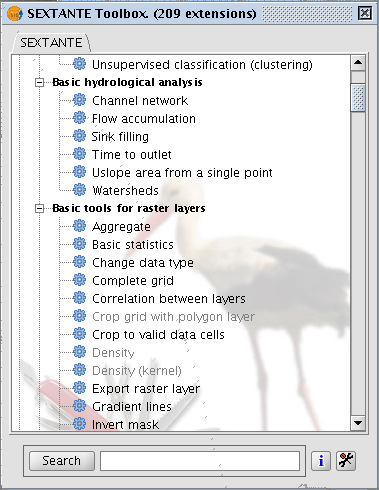
\includegraphics[width=.9\columnwidth]{ExtensionManager.png}
\caption{The SEXTANTE toolbox}
\label{Fig:ExtensionManager}
\end{figure}

	\item The \emph{Graphical Modeller}. Extensions can be used to define a global process than involve several single processes, each of them consisting of a geoalgorithm. Relation between those processes can be defined so the input of one of them can be the output of a previous one, thus setting a workflow. All this is done through a intuitive interface that we will see shortly.
	\item The \emph{Command Line Interface}. A built-in command line for advanced users, which gives more flexibility and allows for the creation of small scripts. 
	\item The \emph{Command History Manager}. Whenever a SEXTANTE extension is run, a new element is added to the SEXTANTE history. Using this element, the command history can be browsed and certain actions can be repeated, just double clicking on a single command or selecting a block of them (Figure \ref{Fig:History}).

\begin{figure}[!hbt]
 \centering
 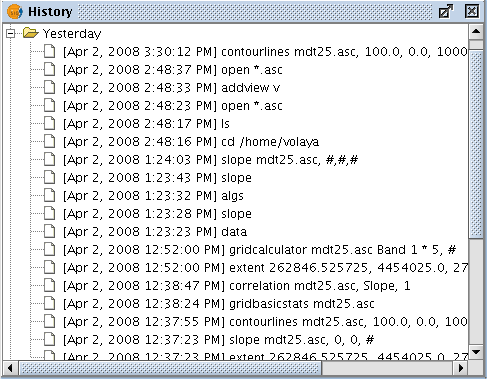
\includegraphics[width=.9\columnwidth]{History.png}
 \caption{Commands can be re--run using the history manager}
\label{Fig:History}
\end{figure}

\end{itemize}

A toolbar with five buttons gives access to all these elements\footnote{Depending on the implementation, access to SEXTANTE elements can also be done via menu items} (Figure \ref{Fig:Toolbar}).

\begin{figure}[!hbt]
 \centering
 
\includegraphics[width=.3\columnwidth]{Toolbar.png}
\caption{The SEXTANTE toolbar}
\label{Fig:Toolbar}
\end{figure}

\section{Executing a single algorithm}

Running a single algorithm is as easy as double clicking on its name in the SEXTANTE toolbox. A new window will appear, which is automatically generated based on the requirements of the algorithm you are going to execute. However, it is easy to define a different interface if needed, as is shown in figure \ref{Fig:ParametersWindow}. 

\begin{figure*}[!hbt]
 \centering
 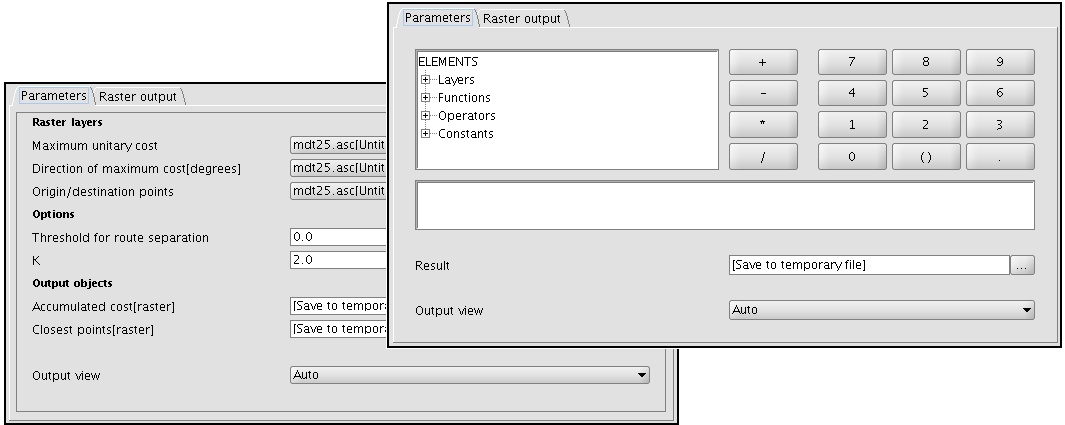
\includegraphics[width=.9\textwidth]{ParametersWindow.png} 
\caption{Parameters windows are automatically generated, but can be easily modified to adapt them to a particular extension}
\label{Fig:ParametersWindow}
\end{figure*}

A tab named \emph{Parameters} allows the user to select or enter the input data (layers, tables, numerical values, strings...). New layers and tables are saved by default to a temporary folder. The user can enter a filepath in case he wants to store an output object permanently.

When the algorithm generates raster layers, a second tab named \emph{Raster output} (Figure \ref{Fig:RasterOutput}) is found as well. Using this tab, the user can set the extent and cell size for all raster layers generated by the algorithm. 

\begin{figure}[!hbt] 
 \centering
 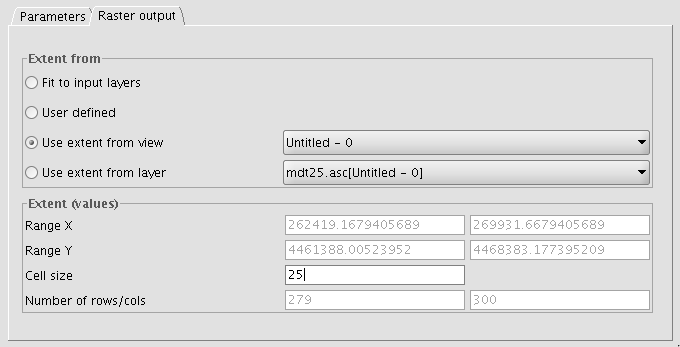
\includegraphics[width=.5\textwidth]{RasterOutput.png}
\caption{The raster output tab}
\label{Fig:RasterOutput}
\end{figure}

Most GIS which include raster analysis capabilities need layers to have the same raster output and cellsize in order to combine them. Some GIS, like GRASS, require the user to define an output region. In SEXTANTE, this region is defined each time the extension is executed, and the user can enter the corresponding values manually, select them from an existing layer, select them from the extent of a view, or let SEXTANTE adjust it  automatically based on the input layers characteristics. This last method is the one selected by default, so most of the time there is no need to use the raster output tab, since the default behaviour is the same as one could expect from any other GIS (specially if there is a single input layer, since the output layers will have its same characteristics)

With this philosophy, data from different sources can be seamlessly integrated to run a process, and the user does not have to worry about preparing those data beforehand. Moreover, preparation of data involves resampling techniques that most users really do not understand enough, being an error prone procedure. Since those resampling tasks are carried on by SEXTANTE, the developer of each algorithm is responsible of how resampling methods are used, so he can let the user select which of them to use or, in most cases, hardcoding it to better fit the algorithm.

Context help for each extension is available, and can be accessed from the dialog box. Users can edit these help files to enhance them or add comments, using the built--in authoring tools (Figure \ref{Fig:HelpAuthoring}). These tools guarantee that help files have the right structure and semantics to be used in different contexts within SEXTANTE, such as the command--line interface that we will later see.

\begin{figure*}[!hbt] 
 \centering
 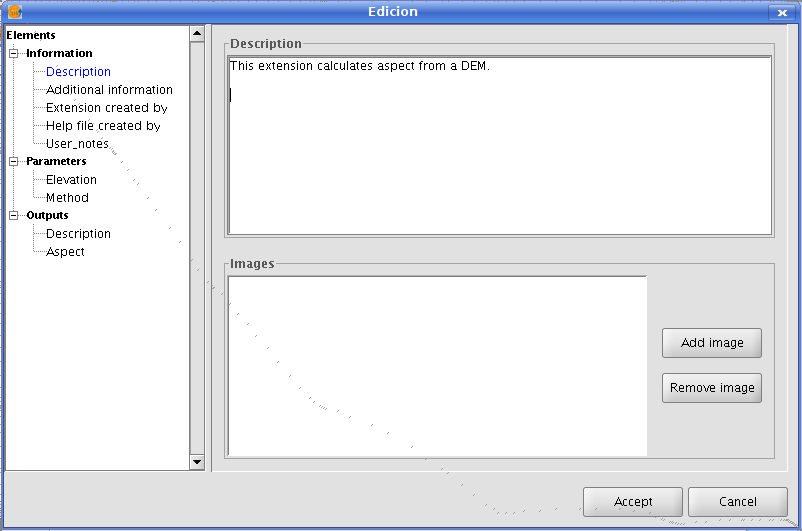
\includegraphics[width=.7\textwidth]{HelpAuthoring.png}
\caption{Help files can be edited using the built--in help--authoring tools}
\label{Fig:HelpAuthoring}
\end{figure*}

Context help can be accessed also directly from the SEXTANTE toolbox, and the whole set of algorithms can be filtered using keywords, so as to make it easier to find the right extension in each case. 

\section{Creating a model}

When working with a GIS, it is frequent to perform calculations that involve several steps. For example, the \emph{Topographic Wetness Index} is defined by \cite{TOPMODEL} as

\begin{equation}
TWI=\ln (a'/\tan \beta)
\end{equation}

\noindent where $a'$ is the upslope contributing area and $\beta$ is the slope.

Therefore, calculating this index in a GIS implies calculating a slope layer from a DEM, an upslope contributing area also from a DEM, and then combining both of them. A great improvement in productivity would be obtained if a user could easily and graphically define a single process that included all this steps, and could execute them all at once.

While proprietary GIS contain such tools (e.g. \emph{ModelBuilder} in ESRI ArcGIS or \emph{MacroModeller} in IDRISI) no free GIS has a similar functionality. GRASS commands can be used to create scripts and define compound processes, but most users find it not user--friendly, and would prefer a graphical interface. Attempts have been made to integrate GRASS with scientific workflow systems such as Kepler (see \cite{GrassKepler}), but the complexity of the resulting solution is way beyond the skills of an average (or even advanced) GIS user.

SEXTANTE includes a graphical modeller which is unique in the FOSS4G scene, allowing users to quickly and effectively create a model, just following two steps:

\begin{itemize}
	\item Defining the inputs needed by the model
	\item Defining the processes to run. Data for each process is introduced through a window similar to the one shown when executing the corresponding extension as a single process. In this case, however, instead of selecting input data from the current gvSIG projects, they are selected from the model inputs (defined in the previous step) and the outputs generated by other processes, thus defining a global workflow.	
\end{itemize}

Figure \ref{Fig:Model} shows the main window of the model builder, with an example model. On the right side of the window, two tabs are found: \emph{Inputs} and \emph{Processes}. Double clicking on their elements, these can be added to the model to define its structure.

\begin{figure*}[!hbt]
 \centering
 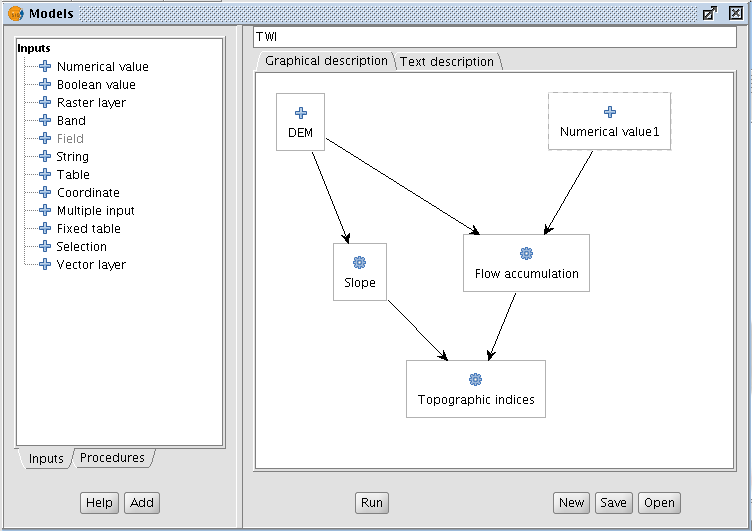
\includegraphics[width=.7\textwidth]{Model.png}
\caption{The graphical modeller window, with an example model}
\label{Fig:Model}
\end{figure*}

Models are saved in XML--based files, and can be easily shared between users.

Once it has been created, the model is treated just as another SEXTANTE algorithm, as if it had been developed directly programming it. It can be run straight from the model builder or incorporated to the algorithms' tree of the toolbox (just saving it to a user--defined models folder), and executed from there as a single process or a batch process, as we will see next.

Models can also have their own context help, which can be edited using the help authoring tools of SEXTANTE.

\section{Executing an extension as a batch process}

All SEXTANTE algorithms (including models) may be executed as batch processes. That is, they can be executed repeatedly on a group of entry parameters without the need of calling each time the corresponding extension through the extension manager.

This can be used, among other things, to execute one operation (for example, the application of a filter) on a group of layers, like, for instance, all the ones in a given folder.

Executing a batch process is not really different from executing a SEXTANTE algorithms in the usual way. The user just has to set the parameters needed to run the corresponding algorithm, and its inputs and outputs. These tasks are done using a table similar to the one shown in figure \ref{Fig:BatchProcess}. 

\begin{figure} [!hbt]
 \centering
 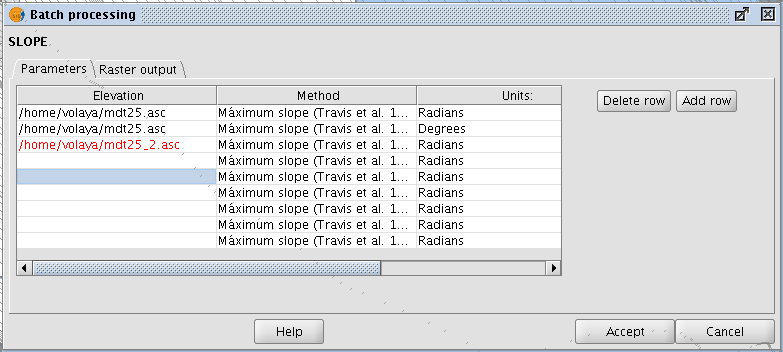
\includegraphics[width=\columnwidth]{BatchProcess.png}
\caption{The batch processing window}
\label{Fig:BatchProcess}
\end{figure}

Each line of the table  represents  an individual execution of the algorithms and the cells of this line contain the values of the parameters, in the same way as they would have been introduced in the different fields of the usual parameters panel.

Inputs are not taken from the GIS directly, but directly from data sources (files). Output layers are not added to the GIS interface, but just saved to the selected filepath.

In order to make it easier to process large sets of files, several additional functionalities have been added, such as automatic completion of output filepaths using a predefined schema (an enumeration, or the value of an input field) and intelligent copy--paste features). Parameters sets can be saved as comma--separated values, and later opened.

\section{Using the command--line interface}

Although most users will prefer using the graphical interface, the command--line interface provides a powerful way of running SEXTANTE extensions (Figure \ref{Fig:CommandLine}). When a certain task is repeated frequently, it is easier and more productive to use the command--line interface instead of the toolbox.

\begin{figure} [!hbt]
 \centering
 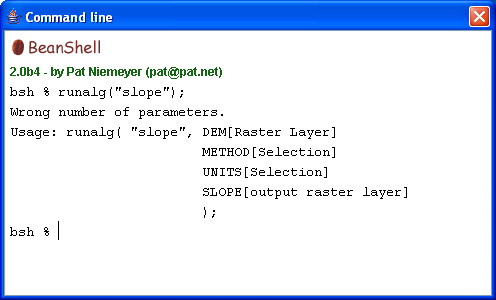
\includegraphics[width=.8\columnwidth]{CommandLine.png}
\caption{The command--line interface}
\label{Fig:CommandLine}
\end{figure}

Scripts can be written and run from the SEXTANTE interface. They can incorporate standard Java elements such as variables, conditional sentences or loops, since the command--line interface is based on the free Java interpreter BeanShell. Additional commands have been added to allow the execution of SEXTANTE geoalgorithms from it.

Scripts can be used to create models and describe compound processes, but there is not yet a link between scripts and models created using the graphical model builder.

\section{Sextante as a WPS actor}

Though OGC's WPS specification provides a mechanism for remote processing and is already fully functional (version 1.0 is already published), current implementations are not practical, mainly due to the lack of processing libraries. In this context, SEXTANTE can play an important role, coupled with WPS servers, enriching them with its comprehensive set of geoalgorithms. 

SEXTANTE has already been incorporated as part of the 52N WPS server, which now can serve a large set of SEXTANTE--based processes. This represents a big step ahead, and opens many new possibilities, specially for WPS clients, since now they have a full--fleged real--world WPS server against which they can operate.

SEXTANTE itself also contains a WPS client as part of its graphical components. This client can wrap WPS processes and turn them into SEXTANTE processes (algorithms that comply with the definition of a geoalgorithm in SEXTANTE), and these can thus be used as local algorithms. This way, WPS processes can be executed as single processes, as batch processes, or incorporated into a model in the SEXTANTE graphical modeller. 

The SEXTANTE WPS client can execute all SEXTANTE algorithms served by a SEXTANTE--based 52N server. In other words an \emph{empty} SEXTANTE (with no local algorithms) can have the same functionality as a \emph{normal} SEXTANTE distribution, accesing all algorithms remotely. This constitutes the ultimate test for the WPS server-client architecture.


\section{The community}

Although SEXTANTE is a small project (three people with just one developer), the community built around it is considerable large, mainly due the increasing popularity of gvSIG and the effort made by the gvSIG team to promote SEXTANTE along with their own software.

Changing from a gvSIG--based conception to an independent library has remarkably increased the number of developers using SEXTANTE. Despite having a large community of users, there was not a large developers community before, something that is gradually changing as more applications start using SEXTANTE as their source of geospatial algorithms.

Developers can access SEXTANTE source code using our SVN repository\footnote{see \url{https://svn.forge.osor.eu/svn/sextante}}, to get a daily updated version. 


\section{More information}

For further information, please visit our website at \url{http://www.sextantegis.com} or send an email to \url{volaya@unex.es} with your questions.

\begin{thebibliography}{2}
\bibitem{GrasKepler}Zhang, J.; Pennington, D.; Michener, W. K. \emph{Automatic Transformation from Geospatial Conceptual Workflow to Executable Workflow Using GRASS GIS Command Line Modules in Kepler}. First International Workshop on Workflow Systems in e-Science (WSES06). Springer Lecture Notes in Computer Science. Volume 3993/2006. 
\bibitem{TOPMODEL} Beven, K. J. \& Kirkby, M. J. (1979) \it{A physically based, variable contributing area model of basin hydrology}, Hydrol. Sci. Bull. 24, 43--69.
\end{thebibliography}

\end{document}